\documentclass[kulak]{tplt} 
% options: kulak (default) or kul

\title{Algebraic Methods in Combinatorics}
\author{Assignment 0}
\date{Summer semester 2022 -- 2023}
\address{
	\textbf{Max Planck Institute for the Mathematics in the Sciences} \\
	\textbf{Universit\"at Leipzig}}


\usepackage{graphicx}
\usepackage{amssymb}
\usepackage{amsthm}
\usepackage{bbold}
\usepackage{listings}
\usepackage{lineno}
%\usepackage[margin=3cm]{geometry}
\usepackage[all,cmtip, color,matrix,arrow]{xy}
%\usepackage{amsaddr}
\usepackage{tikz-cd}
\usepackage{amsmath}%To use \text 
\usepackage[utf8]{inputenc}
\usepackage{hyperref}
\usepackage[capitalize]{cleveref}
\crefname{thm}{Theorem}{Theorems}
%\usepackage{bbold}
\usepackage[export]{adjustbox}
\usepackage{todonotes}
\usepackage{bm}
\usepackage{wrapfig}
\usepackage{float}
\usepackage{mathtools}
\usepackage{aliascnt}
\newaliascnt{eqfloat}{equation}
\newfloat{eqfloat}{h}{eqflts}
\floatname{eqfloat}{Equation}
\usepackage{dirtytalk}
\usepackage[mathscr]{euscript}


%\def\shuffle{\sqcup\mathchoice{\mkern-7mu}{\mkern-7mu}{\mkern-3.2mu}{\mkern-3.8mu}\sqcup\,}
\newcommand{\qshuffle}{\overline{\shuffle}}


\theoremstyle{definition}
\newtheorem{thm}{Theorem}[section]
\newtheorem{prop}[thm]{Proposition}
\newtheorem{lm}[thm]{Lemma}
\newtheorem{cor}[thm]{Corollary}
\newtheorem{obs}[thm]{Observation}
\newtheorem{defin}[thm]{Definition}
\newtheorem{smpl}[thm]{Example}
\newtheorem{quest}[thm]{Question}
\newtheorem{exe}[thm]{Exercise}
\newtheorem{const}[thm]{Construction}
\newtheorem{prob}[thm]{Problem}
\newtheorem{conj}[thm]{Conjecture}
\newtheorem{rem}[thm]{Remark}
\crefname{lm}{Lemma}{Lemmas}
\crefname{thm}{Theorem}{Theorems}
\crefname{prop}{Proposition}{Propositions}
\crefname{defin}{Definition}{Definitions}
\crefname{rem}{Remark}{Remarks}

\newcommand{\R}{\mathbb{R}}
\newcommand{\Z}{\mathbb{Z}}
\newcommand{\F}{\mathbb{F}}
\newcommand{\Q}{\mathbb{Q}}
\newcommand{\PP}{\mathbb{P}}

\newcommand{\one}{\mathbb{1}}

\newcommand{\CC}{\mathcal C}
\newcommand{\JJ}{\mathcal J}
\newcommand{\II}{\mathcal I}
\newcommand{\FF}{\mathcal F}

%vectors
\newcommand{\vv}{\mathsf{v}}
\newcommand{\vw}{\mathsf{w}}
\newcommand{\vj}{\mathsf{j}}
\newcommand{\vx}{\mathsf{x}}
\newcommand{\vy}{\mathsf{y}}
\newcommand{\va}{\mathsf{a}}

\newcommand{\spn}{\mathrm{span}}
\newcommand{\rk}{\mathrm{rk}}
\newcommand{\tr}{\mathrm{tr}}
\newcommand{\conv}{\mathrm{conv}}
\newcommand{\maxcut}{\mathrm{maxcut}}
\newcommand{\we}{\mathrm{we}}


\begin{document}

\maketitle
\begin{enumerate}
\item Eventown and Oddtown

\begin{itemize}
\item In the mountains of Saxony there is a little town called \textbf{Eventown}.
It is a small village with only 10 people.
The people in this village like to form clubs.
What is the maximal amount of clubs that we can have, if we require all of the clubs to have even size?

\item Closeby the arch enemy village sits, \textbf{Oddtown}.
This village also has 10 people and they also like to form clubs. 
What is the maximal amount of clubs that we can have, if we require all of the clubs to be of odd size.
\end{itemize}

\item Colouring the plane

Consider colouring the points in $\R^2$, in such a way that any two points at distance 1 have different colours.
By analysing an equilateral triangle, one can observe that this is impossible to do using only two different colours.
Show that it is also impossible to do such a colouring with three colours, by analysing a larger diagram. 
Show that we can do the colouring with seven colours.

\item Peterson graph

A \textbf{graph} is a pair $(V, E)$ consisting of a ground set $V$ and an edge set $E$, each edge being a collection of two vertices, called its endpoints.
We assume that all graphs are \textbf{simple}, that is no two edges have the same endpoints, and any edge has exactly two distinct endpoints.
An example of such a graph is the Petersen graph, shown in \cref{fig:pet}.

\begin{figure}[h]
\centering
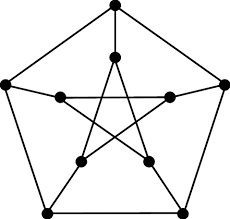
\includegraphics[scale=0.5]{../imgs/petersen.png}
\caption{The Petersen graph\label{fig:pet}}
\end{figure}


The \textbf{degree} of a vertex $v$ is the number of edges that have $v$ as one of its endpoints.
The \textbf{girth} of a graph is the size of the smallest proper cycle.
For instance, any vertex of the Petersen graph has degree three, and the graph has girth five.

Show that a graph of girth five, where all vertices have the same degree $r$, has at least $1+r^2$ vertices.

\end{enumerate}
\end{document}
